\documentclass[11pt]{standalone}

\usepackage{helvet}
\usepackage{units}
\usepackage{textcomp}

\usepackage{ifthen}
\usepackage{tikz} 
\usetikzlibrary{shapes.misc}
\usetikzlibrary{arrows,arrows.meta}
\usetikzlibrary{calc,intersections, patterns, math}
\usetikzlibrary{decorations.pathmorphing}
\usetikzlibrary{shapes.geometric}

\definecolor{pfeil}{RGB}{168,167,167}
\definecolor{petrol}{RGB}{0, 118, 136}
\definecolor{darkgoldenrod}{RGB}{184, 134, 11}
\colorlet{petrol-lighter}{petrol!40}
\colorlet{darkgoldenrod-lighter}{darkgoldenrod!40}

\newcommand{\polygon}[3]{ 
    % #1 = position
    % #2 = anzahl ecken
    % #3 = farbe 
    \pgfmathsetmacro{\MyRand}{3.6*random(0,100)}
    \node[#3, fill,regular polygon,draw,
	regular polygon sides = #2, rotate=\MyRand] at (#1) {\phantom{.}};
}

\begin{document}

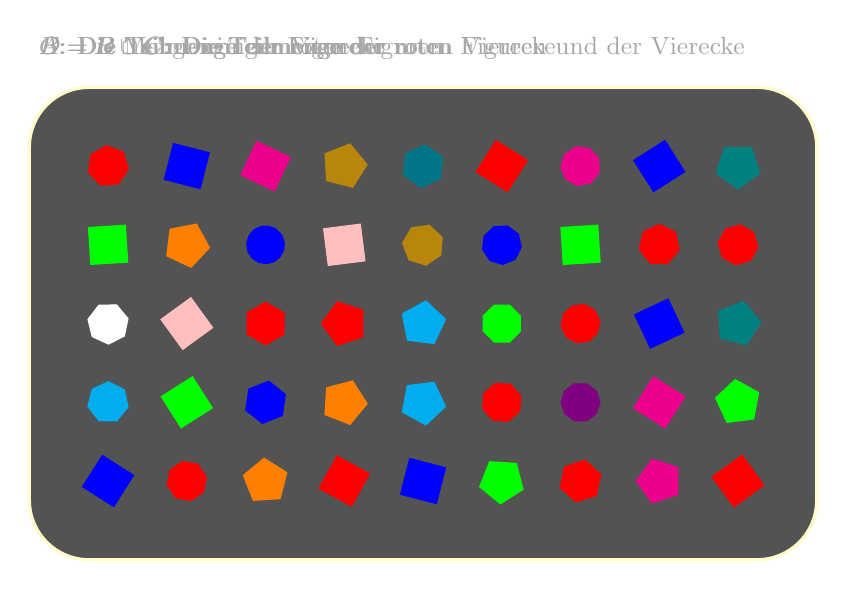
\begin{tikzpicture}[pfeil] 
   

    % \draw[thick, fill=petrol!20, draw=petrol-lighter, rounded corners=2ex, opacity=0.5] (0,0) rectangle ++ (1.5,3.5);
    % \draw[thick, fill=darkgoldenrod!20, draw=darkgoldenrod-lighter, rounded corners=2ex, opacity=0.5] (5,0) rectangle ++ (1.5,3.5);

    \node[right] at (0,6.5) { \small$A$: Die Menge einiger Figuren};
    \node[right] at (0,6.5) { \small$B$: Die Teilmenge der Vierecke};
    \node[right] at (0,6.5) { \small$C$: Die Teilmenge der roten Figuren};
    \node[right] at (0,6.5) { \small$D = B \cap C$: Die Teilmenge der roten Vierecke};
    \node[right] at (0,6.5) { \small$E = B \cup C$: Die Teilmenge der roten Figuren und der Vierecke};

    \draw[very thick, yellow!20, fill=pfeil!50!black, rounded corners = 5ex] (0,0) rectangle (10,6);

    \polygon{1,1}{4}{blue}

    \polygon{2,1}{8}{red}

    \polygon{3,1}{5}{orange}

    \polygon{4,1}{4}{red}

    \polygon{5,1}{4}{blue}

    \polygon{6,1}{5}{green}

    \polygon{7,1}{6}{red}

    \polygon{8,1}{5}{magenta}

    \polygon{9,1}{4}{red}

    %
    %
    %

    \polygon{1,2}{7}{cyan}

    \polygon{2,2}{4}{green}

    \polygon{3,2}{6}{blue}

    \polygon{4,2}{5}{orange}

    \polygon{5,2}{5}{cyan}

    \polygon{6,2}{8}{red}

    \polygon{7,2}{10}{violet}

    \polygon{8,2}{4}{magenta}

    \polygon{9,2}{5}{green}

    %
    %
    %

    \polygon{1,3}{7}{white}

    \polygon{2,3}{4}{pink}

    \polygon{3,3}{6}{red}

    \polygon{4,3}{5}{red}

    \polygon{5,3}{5}{cyan}

    \polygon{6,3}{8}{green}

    \polygon{7,3}{10}{red}

    \polygon{8,3}{4}{blue}

    \polygon{9,3}{5}{teal}

    %
    %
    %

    \polygon{1,4}{4}{green}

    \polygon{2,4}{5}{orange}

    \polygon{3,4}{15}{blue}

    \polygon{4,4}{4}{pink}

    \polygon{5,4}{7}{darkgoldenrod}

    \polygon{6,4}{9}{blue}

    \polygon{7,4}{4}{green}

    \polygon{8,4}{7}{red}

    \polygon{9,4}{8}{red}

    %
    %
    %

    \polygon{1,5}{7}{red}

    \polygon{2,5}{4}{blue}

    \polygon{3,5}{4}{magenta}

    \polygon{4,5}{5}{darkgoldenrod}

    \polygon{5,5}{6}{petrol}

    \polygon{6,5}{4}{red}

    \polygon{7,5}{9}{magenta}

    \polygon{8,5}{4}{blue}

    \polygon{9,5}{5}{teal}

    % \begin{scope}[scale=0.8,decoration={random steps,segment length=2mm}]
    %     \node[rectangle,draw,decorate] at (-2,0) {$\unit[4]{\text\texteuro}$};
    % \end{scope}
    




\end{tikzpicture}




\end{document}
